\documentclass[border=10pt]{standalone}
\usepackage{verbatim}
\usepackage{pgfplots}
\pgfplotsset{compat=1.14}

% stars_count = 512;
% max_time = 2.5
% steps = {0.1, 0.1 / 8, 0.1 / (8 * 8), 0.1 / (8 * 8 * 8), 0.1 / (8 * 8 * 8 * 8)};

\begin{document}

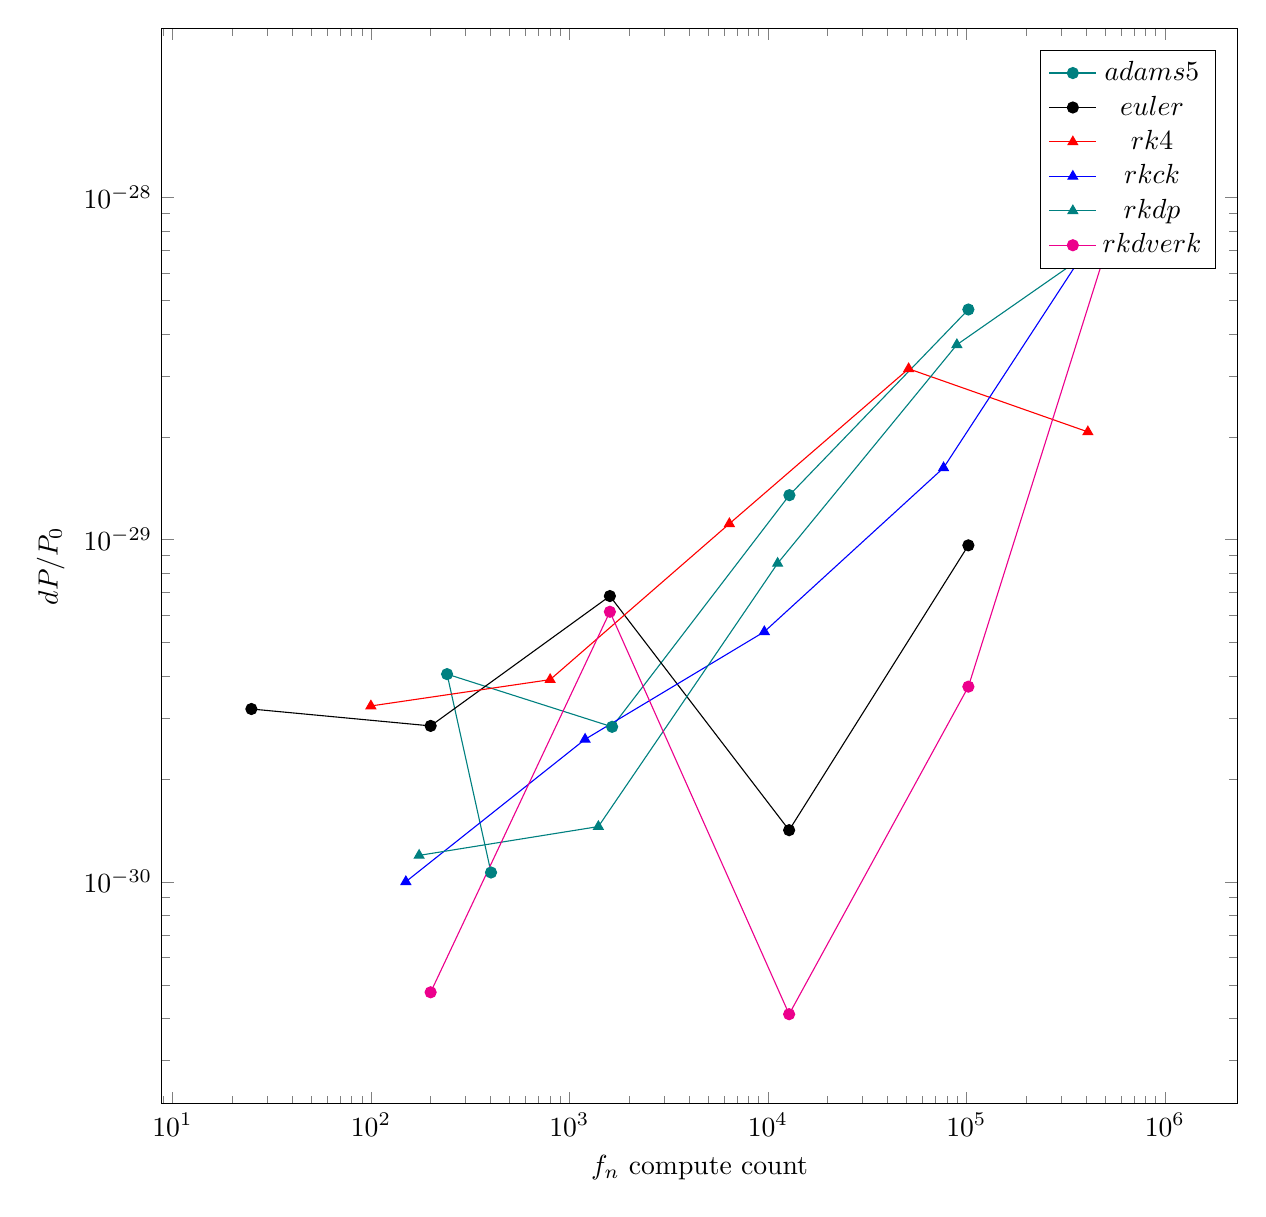
\begin{tikzpicture}
\begin{loglogaxis}[
    height=6in,
    width=6in,
    xlabel=$f_n$ compute count,
    ylabel=$dP/P_0$
]
\addplot [teal,mark=*,solid] coordinates { (403, 1.065e-30) (242, 4.048e-30) (1642, 2.839e-30) (1.284e+04, 1.35e-29) (1.024e+05, 4.711e-29) };
\addplot [black,mark=*,solid] coordinates { (25, 3.201e-30) (200, 2.857e-30) (1600, 6.847e-30) (1.28e+04, 1.416e-30) (1.024e+05, 9.632e-30) };
\addplot [red,mark=triangle*,solid] coordinates { (100, 3.267e-30) (800, 3.901e-30) (6400, 1.114e-29) (5.12e+04, 3.161e-29) (4.096e+05, 2.067e-29) };
\addplot [blue,mark=triangle*,solid] coordinates { (150, 1.001e-30) (1200, 2.61e-30) (9600, 5.384e-30) (7.68e+04, 1.623e-29) (6.144e+05, 1.03e-28) };
\addplot [teal,mark=triangle*,solid] coordinates { (175, 1.195e-30) (1400, 1.451e-30) (1.12e+04, 8.532e-30) (8.96e+04, 3.717e-29) (7.168e+05, 8.615e-29) };
\addplot [magenta,mark=*,solid] coordinates { (200, 4.755e-31) (1600, 6.159e-30) (1.28e+04, 4.103e-31) (1.024e+05, 3.721e-30) (8.192e+05, 1.71e-28) };
\legend{$adams5$,$euler$,$rk4$,$rkck$,$rkdp$,$rkdverk$};
\end{loglogaxis}
\end{tikzpicture}

\end{document}
